\documentclass{ctexart}
\usepackage{graphicx}
\usepackage{caption}
\usepackage{float}
\usepackage{amsmath}
\usepackage{fancyhdr}
\usepackage{xunicode-addon}
\usepackage{booktabs}
\usepackage[a4paper,hmargin=1.25in,vmargin=1in]{geometry}
% !TeX program = xelatex
\title{\begin{figure}[H]
	\centering 
	\includegraphics[height=7cm,width=14cm]{E:/Pictures/中科大.jpg}
	\end{figure}\Huge\textbf{Lab 3}\\\huge{反幂法求按模最小特征值及特征向量}}
\date{}
\punctstyle{banjiao} 
\pagestyle{fancy}
	\fancyhead[C]{\LARGE\textbf{Lab 3}}
	\fancyhead[L]{}
	\fancyhead[R]{}
	\fancyfoot[C]{\thepage}
\begin{document}
	\maketitle
	\thispagestyle{empty}
	
	\[\makebox{\Large{姓名:\underline{\makebox[5cm]{高茂航}}}}\]
	
    \[\makebox{\Large{学号:\underline{\makebox[5cm]{PB22061161}}}}\]
	
	$$\makebox{\Large{日期:\underline{\makebox[5cm]{2024.3.28}}}}$$
	
	\clearpage

	\pagenumbering{arabic}
	\section{Problem Descriptions}
	实现带规范方法的反幂法,求得给定矩阵按模最小特征值以及相应的特征向
	量。
	\section{Analysis and Algorithms} 
	 \subsection{LU-Doolittle分解}
$$\mathbf{A}=\mathbf{L}\mathbf{U}$$
其中$\mathbf{L}$为单位下三角阵,$\mathbf{U}$为上三角阵.
则$\mathbf{A}\mathbf{x}=\mathbf{b}$可化为$$\mathbf{L}\mathbf{U}\mathbf{x}=\mathbf{L}\mathbf{y}=\mathbf{b}$$
只需解方程组
$$\mathbf{L}\mathbf{y}=\mathbf{b}$$
$$\mathbf{U}\mathbf{x}=\mathbf{y}$$
\subsection{规范化反幂法}
$$
 \begin{cases} 
\mathbf{Y^{(k)}} =\mathbf{X^{(k)}}/\|\mathbf{X^{(k)}}\|_{\infty}, \\
\mathbf{A}\mathbf{X^{(k+1)}}=\mathbf{Y^{(k)}},
\end{cases}
k=0,1,…
$$
$\|\mathbf{X^{(k+1)}}\|-\|\mathbf{X^{(k)}}\|_{\infty}\leq10^{-5}$时停止迭代,则$\mathbf{A}$的按模最小特征值$\lambda=1/\|\mathbf{X^{(k+1)}}\|$,$\lambda$对应的特征向量为$\mathbf{Y^{(k)}}$.

\section{Results}

\begin{figure}[H]
	\centering 
	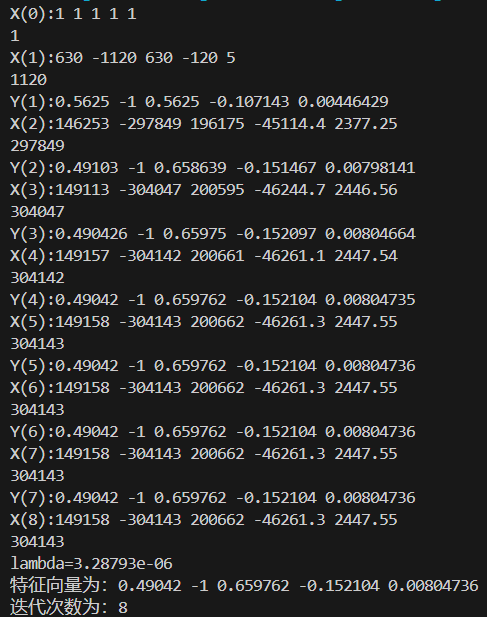
\includegraphics[height=10cm,width=8cm]{1.png}
    \caption{A1的结果}
	\end{figure}
	\begin{figure}[H]
		\centering 
		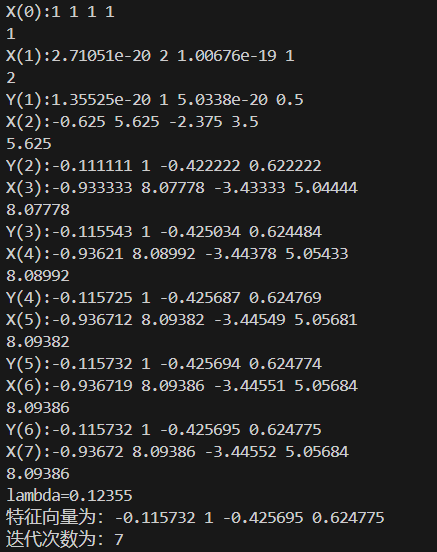
\includegraphics[height=9.5cm,width=8cm]{2.png}
        \caption{A2的结果}
		\end{figure}
		
	\section{Conclusion}
    (a) 本实验中按模最小特征值越接近于0的矩阵,收敛更慢,因此无法直接根据按模最小特征值的大小比较收敛速度,
	可能也和初始向量、最小两个特征值的比值等因素有关。
    
    (b)由于本题矩阵阶数较小,且采用了long double类型, 估计每次迭代的特征值这一过程没有遇到明显的问题。
\end{document}